\documentclass[12pt]{IEEEtran}
\IEEEoverridecommandlockouts
\usepackage{fancyhdr}
\usepackage{graphicx}
\usepackage[spanish, es-tabla, es-nodecimaldot]{babel}
% \usepackage[utf8]{inputenc}
\usepackage{csquotes}
\usepackage{wrapfig}
\usepackage[l3]{csvsimple}
\usepackage{array}
\usepackage[calc, spanish]{datetime2}
\usepackage{enumitem}
% \usepackage{multicol}
\usepackage{chemformula}
\usepackage{multirow}
\usepackage{mismath}
\usepackage{adjustbox}
\usepackage{nccmath}
\usepackage{amsmath}
\usepackage{amssymb}
\usepackage{todonotes}
\usepackage{mathtools}
\usepackage{amsfonts,latexsym} % para tener disponibilidad de diversos simbolos
\usepackage{enumerate}
\usepackage{empheq}
\usepackage{derivative}
\usepackage{float}
\usepackage{threeparttable}
\usepackage{ifpdf}
\usepackage{rotating}
\usepackage{stfloats}
\usepackage{tabularray}
\usepackage{url}
% \usepackage[inline]{showlabels}
\usepackage{kantlipsum}
\usepackage{siunitx}
\usepackage{makecell}%To keep spacing of text in tables
\setcellgapes{2pt}%parameter for the spacing in tables
\usepackage{afterpage}
\usepackage[
  sorting=none,
  backend=biber,
  style=ieee,
  % bibstyle = authoryear,
  citestyle=numeric-comp,
]{biblatex}
\usepackage{hyperref}
\usepackage{cleveref}
\crefname{table}{tabla}{tablas} % Table's cross-reference name
\crefname{equation}{ec.}{ecs.} %
\newcommand\crefrangeconjunction{--}
\newcommand\crefpairconjunction{~y~}
\providecommand{\abs}[1]{\lvert#1\rvert}
%%%%%%%%%%%%%%%%%%%%%%%%%%%%%%%%%%%%%%%%%%%
%%% CREAR Y REESCRIBIR ALGUNOS COMANDOS %%%
%%%%%%%%%%%%%%%%%%%%%%%%%%%%%%%%%%%%%%%%%%%
\newcolumntype{P}[1]{>{\centering\arraybackslash}p{#1}}  %% Se crea un nuevo tipo de columna llamada P.
\newcommand{\tabitem}{~~\llap{\textbullet}~~}
\newcommand{\ctt}{\centering\scriptsize\textbf} %%\ctt abrevia el comando \centering\scriptsize\textbf
\newcommand{\dtt}{\scriptsize\textbf} %%\dtt abrevia el comando \scriptsize\textbf
\renewcommand\IEEEkeywordsname{Palabras clave}

%% Crea una lista en dos columnas
\SetEnumitemKey{twocol}{%
  itemsep = 1\itemsep,
  parsep = 0.5\parsep,
  before = \raggedcolumns
  \begin{multicols}{2},
    after =
\end{multicols}}
%%%%%%%%%%%%%%%%%%%%%%%%%%%%%%%%%%%%%%%%%%%

% correct bad hyphenation here
\hyphenation{op-tical net-works semi-conduc-tor} %% Con este comando se especifican como pueden seprarse las sílabas adecuadamente en caso una palabra quede en dos lineas diferentes de texto

\graphicspath{ {figs/} {logos/}}  %%Ruta donde se encuentran las imágenes, que esté vacio indica que las imagenes están dentro de la misma carpeta que contiene el archivo .tex

\sisetup{
  output-decimal-marker = {.},
  uncertainty-mode = separate,
}
% adjust as needed
\addtolength{\footskip}{0\baselineskip}
\addtolength{\textheight}{-1\baselineskip}

%Paquete tikz para hacer diagramas y figuras
\usepackage{tikz}
\usetikzlibrary{arrows}
%\usepackage[spanish,es-noquoting]{babel}

%%%%%%%%%%%%%%%%%%%%%%%%%%%%%%%%
%%%%% INICIO DEL DOCUMENTO %%%%%
%%%%%%%%%%%%%%%%%%%%%%%%%%%%%%%%

\addbibresource{CaracterizacionPeliculaDelgadaAluminioHiPIMSTribologia.bib}

\DTMsavedate{duedate}{2024-03-25}% Año-Mes-Día -> Fecha de entrega
\DTMnewdatestyle{usvardate}{%
  \renewcommand{\DTMdisplaydate}[4]{%
    \DTMMonthname{##2}\nobreakspace% Mes
    \number##1% Año
  }%
  \renewcommand{\DTMDisplaydate}{\DTMdisplaydate}%
}

\DeclareSIUnit{\min}{min}

\begin{document}
%%%%%%%%%%%%%%%%%%%%%%%%%%%%
%%% TÍTULO DEL DOCUMENTO %%%
%%%%%%%%%%%%%%%%%%%%%%%%%%%%

\title{Estudio de películas delgadas de \ch{Al} depositadas por High-Power Impulse Magnetron Sputtering}

%%%%%%%%%%%%%%%%%%%%%%%%%%%
%%%%%%%%% AUTORES %%%%%%%%%
%%%%%%%%%%%%%%%%%%%%%%%%%%%

\author{\IEEEauthorblockN{Jesús Diego Gómez Garnica, Marcos López Merino}\\
  \IEEEauthorblockA{\textbf{Profesor}: Julio César Cruz Cárdenas}\\
\IEEEauthorblockN{\DTMusedate{duedate}}}

%%%%%%%%%%%%%%%%%%%%%%%%%%%
\twocolumn[
  \begin{@twocolumnfalse}
    \maketitle
    \begin{abstract}
        Las películas delgadas de \ch{Al} tienen aplicaciones en dispositivos electrónicos, almacenamiento de energía y recubrimientos protectores. Con el objetivo de estudiar la adherencia y morfología de películas de \ch{Al}, se depositaron sobre sustratos de vidrio y silicio \ch{Si} mediante High-Power Impulse Magnetron Sputtering (HiPIMS). Las películas se caracterizaron mediante perfilometría óptica (OP), microscopía electrónica de barrido (SEM) y pruebas de \emph{scratch} (\emph{Single Point Scratch Testing}). Los resultados mostraron un espesor promedio de \qty{280}{\nm}. Las pruebas de \emph{scratch} revelaron una carga crítica de \qty{0.1}{\N} y \qty{0.5}{\N}, sugiriendo problemas de adherencia. Estos resultados subrayan la de técnicas complementarias para una caracterización adecuada de las películas de \ch{Al} depositadas por esta técnica.
    \end{abstract}

    \begin{IEEEkeywords}
        HiPIMS, SEM, Scratch Test
    \end{IEEEkeywords}
  \end{@twocolumnfalse}
  \vspace{1cm}
]

%https://doi.org/10.1016/j.surfcoat.2022.128409 -> Aplicaciones

%%%%%%%%%%%%%%%%%%%%%%
%\IEEEpeerreviewmaketitle
%%%%%%%%%%%%%%%%%%%%%%%%%%%%%%%%%%%%%
%%% PRIMERA SECCIÓN DEL DOCUMENTO %%%
%%%%%%%%%%%%%%%%%%%%%%%%%%%%%%%%%%%%%
\section{Introducción}

Las películas delgadas son capas de material con espesores que van desde unos cuantos nanómetros hasta varios micrómetros y pueden encontrarse en revestimientos antirreflejantes para anteojos y hasta en chips de computadoras. Su ventaja radica en la combinación de las propiedades superficiales de la película delgada con las propiedades del material subyacente, lo que mejora las características químicas, mecánicas o eléctricas, entre otras. 
Existen múltiples técnicas para producir películas delgadas, tales como electrodeposición (\emph{electroplating}), la evaporación, la pulverización catódica (\emph{sputter deposition}), la deposición química de vapor  (CVD, por sus siglas en inglés) y combinaciones de estas. En este trabajo nos enfocaremos en una técnica recientemente desarrollada llamada \emph{high-power impulse magnetron sputtering} (HiPIMS) \cite{lundinHiPIMSProcess2010}.

HiPIMS es un método de deposición física de vapor (\emph{physical vapor deposition}, PVD) basado en la pulverización catódica con magnetrón (\emph{direct current magnetron sputtering}, DCMS). Esta técnica utiliza densidades de potencias extremedamente altas, del orden de \unit{\kW\per\cm^{2}}, en pulsos cortos de decenas de microsegundos. Las películas delgadas depositadas por esta técnica dan como resultado películas más densas.

Las películas delgadas pueden caracterizarse mediante diversas técnicas para evaluar su crecimiento, calidad, entre otras características. Una de estas es la microscopía electrónica de barrido (\emph{scanning electron microscopy}, SEM), que emplea un haz enfocado de electrones para escanear la superficie de una muestra punto por punto y examinarla con alta resolución. 
La interacción del haz de electrones con la superficie de la muestra da lugar a dos tipos distintos de electrones: electrones retrodispersados (\emph{backscattered electrons}, BSE) y electrones secundarios (SE). Los BSE son electrones de alta energía provenientes del haz incidente del SEM que experimentan dispersión elástica con los núcleos atómicos de la muestra. En contraste, los SE son electrones de bajas energías emitidos desde la superficie cuando es irradiada con el haz de electrones, el cual transfiere su energía a los electrones atómicos a través de colisiones inelásticas que se emiten desde los primeros nanómetros de la superficie de la muestra debido a su limitada profundidad de penetración \cite{WhichElectronDetector2023,infoInterpretingImagesScanning2022}.
Mediante la amplificación de la señal, es posible obtener imágenes topográficas de la superficie de la muestra con facilidad. Además, se pueden obtener imágenes de la sección transversal, lo que permite analizar el grosor de la película y su microestructura.

Una prueba para evaluar las características mecánicas es la prueba de rayado (\emph{scratch}), en la que un contracuerpo (\emph{stylus}), se pone en contacto con la película. La muestra se coloca sobre una plataforma de alta precisión que la pone en contacto con la punta, moviéndola da una velocidad constante y aplicando una carga constante o progresiva. Es una prueba tribológica destinada a evaluar la integridad mecánica, modos de falla y la fuerza de adherencia de un recubrimiento \cite{internationalStandardTestMethod}.

\begin{figure}[htp]
    \centering
    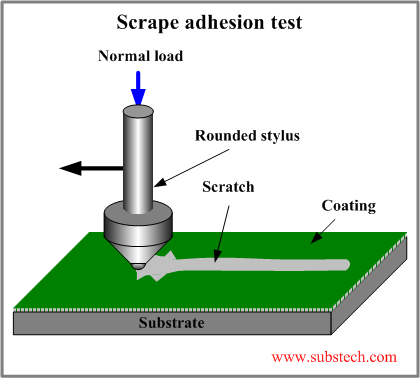
\includegraphics[width=0.8\linewidth]{scratch-test}
    \caption{Esquema de una prueba de rayado. \cite{kopeliovich_adhesion_nodate}}
    \label{fig:scratch-test}
\end{figure}

\section{Procedimiento experimental}

A partir de las películas delgadas de \ch{Al} depositadas en sustratos de \ch{Si} y portaobjetos de vidrio a \todo[inline]{colocar parámetros de depósito}
se hicieron posteriormente pruebas para caracterizar la película delgada, así como medir el espesor del mismo.

\subsection{Medición del espesor}

Para medir el espesor de las películas se colocó una gota de pegamento a uno de los sustratos el cual posteriormente fue retirado, resultando en un cráter de altura igual al grosor de la película delgada, donde se realizó la medición usando la técnica de perfilometría óptica. El perfilómetro óptico utilizado fue el Nexview de la marca ZYGO. 

\subsection{Prueba de \emph{scratch}}

La prueba de \emph{scratch} se realizó usando el tester mecánico NANOVEA CB500 en la película depositada en el portaobjetos de vidrio siguiendo la norma ASTM-1624. Esta se prueba se llevó acabo a una temperatura \qty{22.7}{\degreeCelsius} utilizando un contracuerpo de hierro con cromo de \qty{1}{\mm} aplicando una carga progresiva de \qty{0.01}{\N} hasta \qty{2.5}{\N} y de \qty{0.01}{\N} hasta \qty{1}{\N} con una velocidad constante de \qty{1}{\mm\per\min} en una distancia de \qty{5}{\mm}.

\subsection{SEM}

Para la obtención de las imágenes SEM de la sección transversal y la superficie de la película depositaa en \ch{Si} se usó el microscopio JEOL JSM-6010LA, a una resolucion de 20,000 x y 10,000 x respectivamente.

\section{Resultados y análisis}

El grosor de la película al ser medida desde el perfilómetro óptico resulto no ser constante, este variaba significativamente en un promedio entre $250 nm$ a $300 nm$, esto dificulto tener una fiablilidad al realizar la prueba de scratch.

Al ver la pelicula con una resolucion mayor por medio de un microscopio la pelicula presento zonas irreguales donde no habia recubrimiento, sin embargo se procedio con la prueba, la fractura expuesta fue del tipo adhesiva, el material se abrio sobre la pelicula y parte del mismo quedo sobre el contracuerpo de 1mm de diametro, utilizamos este mismo contracuerpo para realizar la segunda prueba de rayado, en este caso antes de romperse y adherirse al contracuepro este dio saltos sobre la superfie, dejando el coeficiente de friccion con picos significativos

\section{Conclusiones}
\kant[5]


%%%%%%%%%%%%%%%%%%%%%%%%%%%%%%%%
%%%%%%    Bibliografia   %%%%%%%
%%%%%%%%%%%%%%%%%%%%%%%%%%%%%%%%
% \newpage
\nocite{*}
\printbibliography
%\section{Apéndices}
%\appendices

\end{document}
%%%%%%%%%%%%%%%%%%%%%%%%%%%%%%%%
%%%%%% FIN DEL DOCUMENTO %%%%%%%
%%%%%%%%%%%%%%%%%%%%%%%%%%%%%%%%
